\documentclass[11pt]{article}

\usepackage{amsmath}
\usepackage{textcomp}
\usepackage{graphicx}
\usepackage{wrapfig}

\usepackage[top=0.8in, bottom=0.8in, left=0.8in, right=0.8in]{geometry}
\usepackage{listings}
\usepackage{color}

\definecolor{dkgreen}{rgb}{0,0.6,0}
\definecolor{gray}{rgb}{0.5,0.5,0.5}
\definecolor{mauve}{rgb}{0.58,0,0.82}

\lstset{frame=tb,
  language=Java,
  aboveskip=3mm,
  belowskip=3mm,
  showstringspaces=false,
  columns=flexible,
  basicstyle={\small\ttfamily},
  numbers=none,
  numberstyle=\tiny\color{gray},
  keywordstyle=\color{blue},
  commentstyle=\color{dkgreen},
  stringstyle=\color{mauve},
  breaklines=true,
  breakatwhitespace=true,
  tabsize=3
}

% Add other packages here %


\title{\bf Excercise 4\\ Implementing a centralized agent}
\author{Group \textnumero{15} : Christian Sciuto, Lorenzo Tarantino}


% N.B.: The report should not be longer than 3 pages %


\begin{document}
\maketitle

\section{Solution Representation}

\subsection{Variables}
% Describe the variables used in your solution representation %
\begin{enumerate}
\item vehicleActionMap: the key of the map is a vehicle and the value is an object from the Action class, that contains a task and an ActionType = $\{PICKUP, DELIVERY\}$
\item taskActionTimesMap: the key of the map is a task and the value is an object from the ActionTimes class that contains the pickUp and delivery times of that task (of course the task refers to only one vehicle, see below).
\end{enumerate}

\subsection{Constraints}
% Describe the constraints in your solution representation %
\begin{enumerate}
\item loadConstraint(Vehicle vehicle): the total weight of the carried tasks must be lower than the capacity of the vehicle in every moment;
\item timeConstraint(Task task): the time for the pickUp of a task has to be strictly lower than the delivery time of that task;
\item allTasksDeliveredConstraint(): the number of tasks picked up and delivered has to be equal to all the existing tasks;
\item taskUnique(Task task): one task has to be picked up and delivered by one and only one vehicle;
\item actionsAtDifferentTimesConstraint(): every vehicle has to do its actions in different times.
\end{enumerate}

\subsection{Objective function}
% Describe the function that you optimize %
Definition of cost:
\begin{equation*}
    \mathbf{cost(C_1, C_2)} = \mathbf{distance(C_1, C_2) * costPerKm(vehicle)}
\end{equation*}
where $C_n$ is a city, the distance($C_1$, $C_2$) functions returns the distance between the two cities following the shortest path and costPerKm(vehicle) returns the cost per km of that vehicle.
\\
Our objective function computes the total cost of the solution as the sum of the costs per vehicle. The cost per vehicle is computed in the following way: first we add to the total cost the cost from the current position of the vehicle to the city of the first action (that is a pickUp action). Then we loop on the actionList of the vehicle, and for every action we compute the cost from the city of that action to the city of the next one.

\section{Stochastic optimization}

\subsection{Initial solution}
% Describe how you generate the initial solution %
After having tried different methods of initial solutions (random assignment of the tasks, all the tasks to the vehicle with the biggest capacity...), we found that the best initial solution is to first give the tasks that are in the currentCity of one vehicle to that vehicle (until it is full) and then distribute all the remaining tasks one for each vehicle.

\subsection{Generating neighbours}
% Describe how you generate neighbors %
First, new solutions from Solution class are created by changing one random task from a random vehicle to all the other vehicles (one new solution for each vehicle different from the one selected). All the new solutions are added to a neighbor solution list. Secondly, for the random vehicle selected, we change the order of two actions of its actionList, pair-wise for each couple of actions. A new solution is created for every couple of actions swapped. We add the new solutions to the neighbor list. Finally, every solution in the neighbors list is filtered and eliminated if it does not respect all the constraints.
\subsection{Local choice}
Given the set of neighbor solutions, it finds the minimum cost solution in the neighbors list and with a probability p it selects the new one, otherwise it keeps the current solution. At this point we verify the cost of the solution chosen and after minimumThreshold iterations where the solution cost does not change, the method will choose a random solution in the neighbor list. We added the parameter minimumThreshold in order to avoid to remain stuck in a local minimum that maybe is not the best.

\subsection{Stochastic optimization algorithm}
% Describe your stochastic optimization algorithm %
Starting from an initial solution, for each iteration the algorithm creates a list of neighbors solutions of the current one, then it selects a new solution from the neighbor list with the 'localChoice' method. In each steps the global best solution (the one with the minimum cost found in this search) is updated if the new solution chosen has a lower cost.

\section{Results}

\subsection{Experiment 1: Model parameters}
% if your model has parameters, perform an experiment and analyze the results for different parameter values %
We run simulations with different probability parameter and different minimumThreshold.

\subsubsection{Setting}
% Describe the settings of your experiment: topology, task configuration, number of tasks, number of vehicles, etc. %
% and the parameters you are analyzing %
Topology: England.xml; 20 tasks, 4 vehicles and 10000 iterations. We will use probability: [0.35, 5, 1] with fixed minimumThreshold = 50; then minimumThreshold: [50, 500] with probability = 0.35

\subsubsection{Observations}
% Describe the experimental results and the conclusions you inferred from these results %
probability = 0.35 \textrightarrow finalCost = 10831.5; probability = 0.5\textrightarrow finalCost = 11005.0;   probability = 1 \textrightarrow finalCost = 11378.0.
\\
minimumThreshold = 50 \textrightarrow finalCost = 10831.5; minimumThreshold = 500 \textrightarrow finalCost = 13769.0
\\
\\
We can conclude that, given our implementation o the 'localChoice' method, our solutions are more influenced by the minimum threshold parameter ( when we increase it, it is more likely to obtain worst solutions).

\subsection{Experiment 2: Different configurations}
% Run simulations for different configurations of the environment (i.e. different tasks and number of vehicles) %
In this experiment we run simulations for different number of vehicles and different number of tasks. Furthermore, for each test, we run the SLS algorithm with two different implementations of the localChoice method. The first implementation is our 'localChoice' method that we already described, the second implementation was the one suggested in the paper assigned for this exercise.
\subsubsection{Setting}
% Describe the settings of your experiment: topology, task configuration, number of tasks, number of vehicles, etc. %
Topology: England.xml; Task configuration: default from the template.
\\
First, we tried with 20 tasks and three, four and five vehicles respectively. Then we repeated the same procedure for 30 tasks.

\subsubsection{Observations}
% Describe the experimental results and the conclusions you inferred from these results %
% Reflect on the fairness of the optimal plans. Observe that optimality requires some vehicles to do more work than others. %
% How does the complexity of your algorithm depend on the number of vehicles and various sizes of the task set? %

For each configuration (tasks, vehicles) we  run the test 10 times, then we decided to show only the best result. This is because a raw mean of the ten results for each configuration does not represent a reliable data due to the probalistic situation of the problem. 
\\
The next table contains the results obtained using our 'localChoice' implementation:
\small
\begin{center}
    \begin{tabular}{ | l | l | l | l | l |}
    \hline
    \textbf{Tasks} & \textbf{3 Vehicles} & \textbf{4 Vehicles} & \textbf{5 Vehicles}\\ \hline
    20 & (final cost = 9937.0, time = 11 s) & (final cost = 10243.0, time = 9 s) & (final cost = 10685.0, time = 5 s)\\ \hline
    30 & (final cost = 15645.0, time = 20 s) & (final cost = 13832.0, time = 18 s) & (final cost = 14580.0, time = 13 s)\\ \hline
    \end{tabular}
\end{center}
\normalsize
The table below contains the values computed using the 'localChoice' method presented in the paper:
\small
\begin{center}
    \begin{tabular}{ | l | l | l | l | l |}
    \hline
    \textbf{Tasks} & \textbf{3 Vehicles} & \textbf{4 Vehicles} & \textbf{5 Vehicles}\\ \hline
    20 & (final cost = 11418.0, time = 7 s) & (final cost = 12046.0, time = 4 s) & (final cost = 11327.0, time = 3 s)\\ \hline
    30 & (final cost = 15645.0, time = 18 s) & (final cost = 15070.0, time = 12 s) & (final cost = 17781.0, time = 8 s)\\ \hline
    \end{tabular}
\end{center}
\normalsize

\begin{enumerate}
\item We obtain better results for each configutation with our localChoice implementation, this is because 'localChoice' method on the paper is more prone to be stuck in local minimum.
\item On the other hand, our 'localChoice' implementation makes the SLS slower compared to using the 'localChoice' method on the paper. This is because when we try to avoid a local minimum, we select a random solution from the neighbor.
\item We can notice that, when we increase the number of tasks, our algorithm complexity increases (the computational time increases). This was expected because we create more solutions with the 'changingVehicle' and 'swapActions' methods. Also, if we increase the number of vehicles, then our computational time decreases, mostly because we have less tasks per vehicle.
\end{enumerate}
\normalsize
Finally, with this centralized behavior, it is possible to see that sometimes in the best solution some vehicles have more work than others. In this example we had 3 vehicles and 20 tasks in the england topology, we had as final cost: 9937 and computational time: 11 seconds. As you can see in the picture below, the best solution found was to assign the tasks to only two vehicles:
\begin{center}
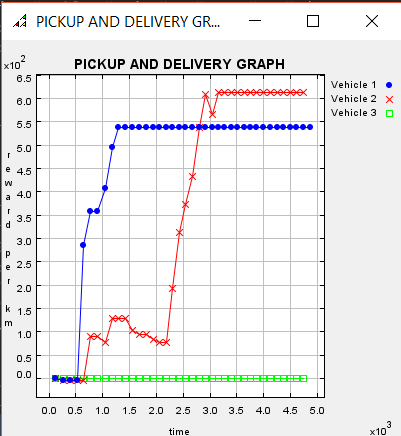
\includegraphics[scale=0.3]{2_vehicl.png}
\end{center}

\end{document}